\chapter{Introducción}

\section{¿Qué es DevOps?}

\enquote{El término \textit{DevOps}, que es una combinación de los términos ingleses \textit{development} (desarrollo) y \textit{operations} (operaciones), designa la unión de personas, procesos y tecnología para ofrecer valor a los clientes de forma constante} \cite{devops}. Gracias a esta práctica y a sus herramientas, los roles que trabajan en el desarrollo del software pueden trabajar juntos para producir productos mejores y más confiables, además de hacer que mejore el rendimiento de los equipos y creen productos de calidad en menos tiempo.

\subsection{Prácticas DevOps}

La mayoría de las prácticas de \textit{DevOps} están diseñadas para agilizar, automatizar y mejorar las fases del desarrollo del software, reduciendo el riesgo de errores humanos y mejorando la velocidad.

\begin{itemize}
	\item \textbf{Integración y Despliegue Continuos (CI/CD).} Mediante la práctica de Integración Continua, cada vez que se fusionan los cambios en la rama de código principal (cada vez que se realiza un \enquote{commit}), se realizan pruebas automáticas para garantizar la estabilidad de la rama principal \cite{devops}.\\
	
	El Despliegue Continuo es la automatización de la puesta en producción de los nuevos cambios y también se ejecuta al fusionar nuevos cambios en la rama principal. De esta forma, es mucho más rápido el proceso del despliegue al no tener que hacerlo manualmente y nos permite realizar implementaciones más frecuentes \cite{devops}.
	
	\item \textbf{Control de versiones.} \enquote{Es la práctica que nos permite administrar el código por versiones y del historial de cambios para facilitar la revisión y la recuperación del código} \cite{devops}. El sistema que nos brinda esta utilidad es \textit{git} y el código suele estar publicado en un repositorio remoto (que puede ser privado o público) usando este mismo sistema para que todo el equipo tenga acceso al control de versiones.
	
	\item \textbf{Infraestructura como Código.} \enquote{Permite definir las topologías y los recusos de un modo descriptivo que permite a los equipos administrar esos recursos igual que lo harían con el código} \cite{devops}. Además, al estar definida como código, se puede administrar sus versiones con el sistema de control de versiones. En adición, hace que la creación de la infraestructura sea repetible y ayuda a automatizar el Despliegue continuo.
	
	\item \textbf{Administración de configuración.} Podemos usarla junto con la Infraestructura como Código para automatizar la definición y configuración de sistemas \cite{devops}. Es muy común guardar la configuración de un sistema en un fichero con un formato determinado (si no contiene información confidencial como contraseñas), como variable de entorno en una única máquina o usar un mecanismo de configuración distribuida si utilizamos un cluster (como por ejemplo etcd \cite{etcd}).
	
	\item \textbf{Monitorización.} Consiste en visualizar en tiempo real el rendimiento y el estado de la pila de aplicaciones, desde la infraestructura subyacente hasta el software de niveles superiores con el fin de mitigar los errores producidos durante la ejecución de la misma o ver si es necesario escalarla \cite{devops}.
\end{itemize}

\subsection{DevOps y contenedores}

\enquote{Los contenedores linux son una tecnología que nos permite empaquetar y aislar aplicaciones junto con su entorno de ejecución (todos los archivos necesarios para que funcione)} \cite{containers}. Esto nos permite que la aplicación se pueda ejecutar en cualquier máquina/arquitectura que ejecute Linux sin problemas (solo se tiene que tener instalado algún \textit{container engine}) y con mucha facilidad, pues los contenedores son portables. Para esto, existe en internet un gran número de repositorios de contenedores, que  nos permite subirlos de manera gratuita y descargarlo en otra máquina. Gracias a esta tecnología, podemos facilitar mucho el flujo de CI/CD al poder ejecutar la aplicación y sus tests en un contenedor.\newline

\section{Motivación para usar MLOps}

Hoy en día, en los proyectos de Machine Learning, el código dedicado a definir los modelos predictivos representa una fracción muy pequeña comparada con otros componentes del flujo de trabajo. Para poder operar con modelos, los científicos de datos deben de trabajar junto con otras personas que se dedican a eso mismo, operaciones (encargados de desplegar, testear el sistema, aprovisionar la infraestructura necesaria, etc). Esto representa un desafío en la organización en términos de comunicación, colaboración y coordinación. El objetivo de MLOps es enfrentarse a dicho desafío estableciendo buenas prácticas para el desarrollo. Además, nos aporta de la velocidad y agilidad necesaria en el mundo digital actual.

\begin{figure}[h]
	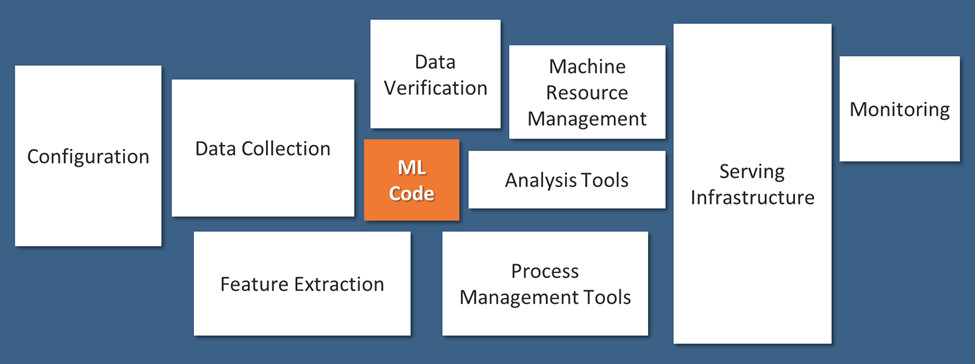
\includegraphics[scale=1]{imagenes/01_Introduccion/mlcodefraction.jpg}
	\centering
	\caption{Como se muestra en la figura, la fracción de código en los sistemas de ML reales es bastante pequeña. En cambio la fracción de infraestructura es mucho mayor \cite{NIPS2015_86df7dcf}.}
\end{figure}

En este caso, adoptar las mejores prácticas de \textbf{DevOps} podría ser posible, pues el Machine Learning tiene mucho en común con la ingeniería del software. La diferencia es que en Machine Learning hay que llevar un registro de modelos y sus hiperparámetros, con el fin de que el experimento se pueda replicar con la mayor facilidad en otro sistema (esto recibe el nombre de reproducibilidad) \cite{whymlops}.\newline

En DevOps y MLOps se debe de usar un sistema de control de versiones (git) para poder gestionar los cambios en el código. Adicionalmente, en MLOps necesitamos registrar los modelos y los hiperparámetros usados para su posterior uso, pero gracias a la herramienta \textit{mlflow} (su uso está explicado en un capítulo posterior) esto ya no es problema. Además de todo lo anterior, el código debe de estar subido a un repositorio remoto compartido (como puede ser GitHub, GitLab, Bitbucket, etc) para poder trabajar cómodamente en equipo. En este repositorio debemos tener el control de que en cada cambio incremental todo lo anterior y lo nuevo siga funcionando, por lo tanto es necesario el uso de lo que se llama Integración Continua. Este proceso de Integración Continua lo que hace es ejecutar los tests que hemos escrito sobre el código implementado para comprobar que efectivamente funciona como esperábamos. En cuanto a MLOps, también es necesario testear que los modelos se comporten como esperamos. Esto nos permite desarrollar software de mayor calidad y con una altísima frecuencia de \textit{releases}.\newline

Además de lo anterior, también se puede configurar un Despliegue Continuo, así si nuestro código pasa con éxito los tests de Integración Continua, podriamos desplegarlo en cuestión de segundos o unos pocos minutos mediante otras herramientas/plataformas que nos permitan acelerar dicho despliegue usando Infraestructura como Código. Para poder integrar la Integración Continua y el Despliegue Continuo (a partir de ahora lo llamaremos CI/CD\footnote{Hay dos conceptos bastante parecidos que pueden llevar a confusión, uno es \textit{Continuous Delivery} y otro es \textit{Continuous Deployment}. El primero se refiere a la automatización del proceso de lanzamiento de \textit{releases} con un solo o varios clicks. El segundo se refiere a la automatización completa del proceso anterior. En este trabajo se busca el desarrollo de un \textit{pipeline} de \textit{Continuous Deployment} \cite{continuous_delivery_deployment}.}) nos hace falta una plataforma en la nube que nos lo permita. Todo esto está desarrollado en los próximos capítulos de este documento.

\section{Descripción del problema}\label{sec:problemdesc}

La Tierra está siendo \enquote{bombardeada} constantemente con rayos cósmicos que provienen, como su nombre indica, del universo. Estos rayos se componen de partículas que viajan a la velocidad de la luz, que al entrar en contacto con la atmósfera producen una cascada atmosférica extensa. Dicha cascada emite una luz debido a la radiación gamma llamada \enquote{Luz de Cherenkov}.\newline

\enquote{La detección de de rayos gamma de muy alta energía es esencial para investigar las fuentes de la radiación entrante producida por alguno de los fenómenos más extremos que suceden en el universo, por ejemplo estrellas de neutrones y agujeros negros supermasivos} \cite{gonzalez2021tackling}.

\begin{figure}[H]
	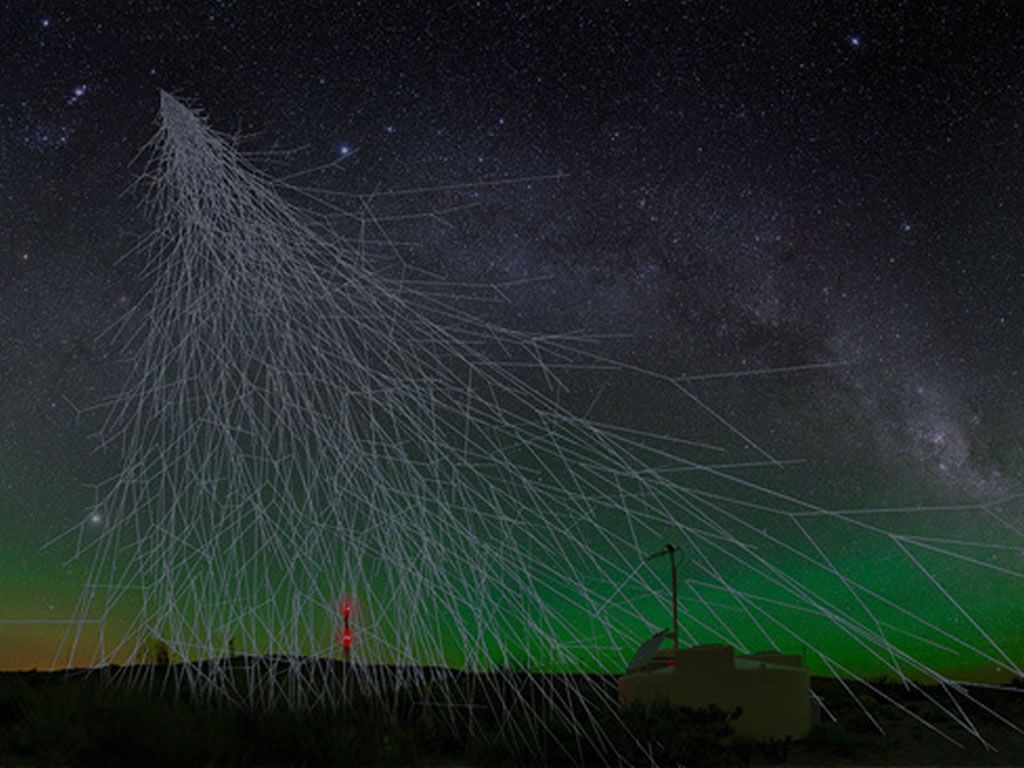
\includegraphics[width=.8\linewidth]{imagenes/01_Introduccion/EAS.jpg}
	\centering
	\caption{Así sería una Cascada Atmosférica Extensa incidiendo sobre un Water Cherenkov Detector (WCD). Fuente: \href{https://revolucion.news/cienciario.mx/los-rayos-cosmicos-de-muy-alta-energia-vienen-de-fuera-de-la-via-lactea/}{revolucion.news}.}
	\label{fig:wcd}
\end{figure}

Para poder capturar información sobre dichos rayos cósmicos, se usan Detectores de agua de Cherenkov (Water Cherenkov Detectors, WCD) que son tanques de agua ultrapura que contienen fotomultiplicadores distribuidos simétricamente, como puede verse en la Figura \ref{fig:wcdschema}, (la cantidad de fotomultiplicadores depende del diseño del tanque) y son utilizados para captar la señal del rayo que incide sobre el mismo. En función de la profundidad del agua del WCD, se emitirá más luz o menos, siendo directamente proporcionales. En la Figura \ref{fig:wcd} podemos observar cómo son desde fuera.\newline

\begin{figure}[H]
	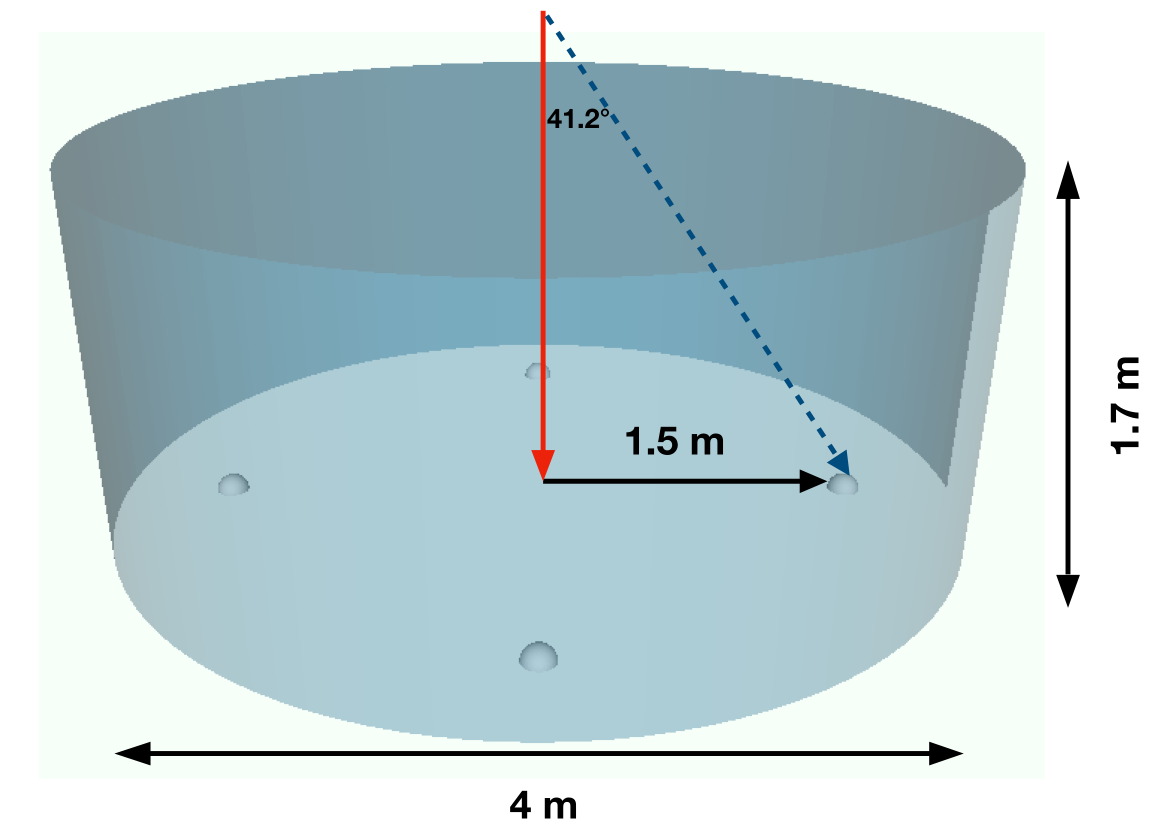
\includegraphics[scale=.1]{imagenes/01_Introduccion/wcd.png}
	\centering
	\caption{Diseño de un WCD \cite{gonzalez2021tackling}.}
	\label{fig:wcdschema}
\end{figure}

El problema que se pretende solucionar en este proyecto, es diseñar un modelo que sea capaz de diferenciar entre dos tipos de cascadas atmosféricas que son producidas por distintas partículas que provienen del universo, las producidos por partículas de hierro y las producidas por protones. Para ello, los datos que tenemos son imágenes de una simulación, en la que podemos observar la cantidad de energía recogida en cada punto. Cada uno de esos puntos representa un WCD. Las dos siguientes imágenes muestran una muestra de las dos clases que tenemos en el conjunto de datos:

\begin{figure}[h]
     \centering
     \begin{subfigure}[b]{0.45\textwidth}
         \centering
         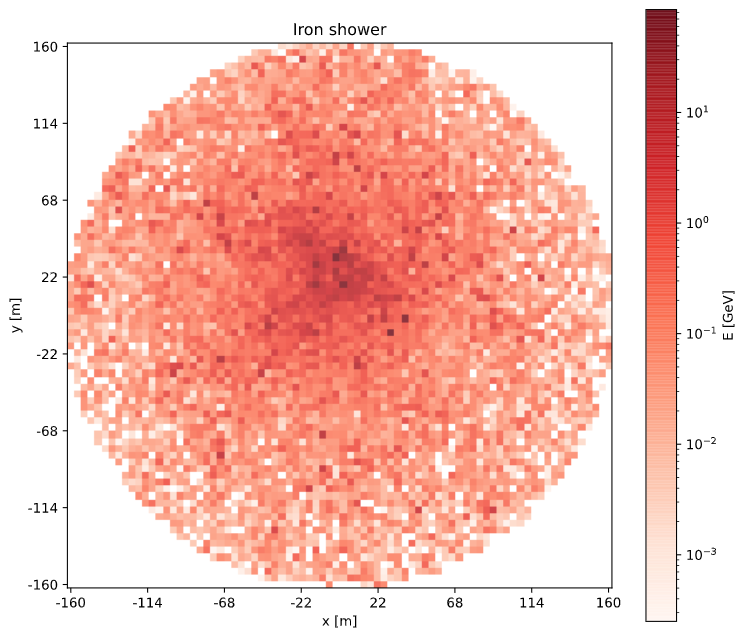
\includegraphics[width=\textwidth]{imagenes/01_Introduccion/iron.png}
         \caption{Cascada generada por hierros}
         \label{fig:y equals x}
     \end{subfigure}
     \hfill
     \begin{subfigure}[b]{0.45\textwidth}
         \centering
         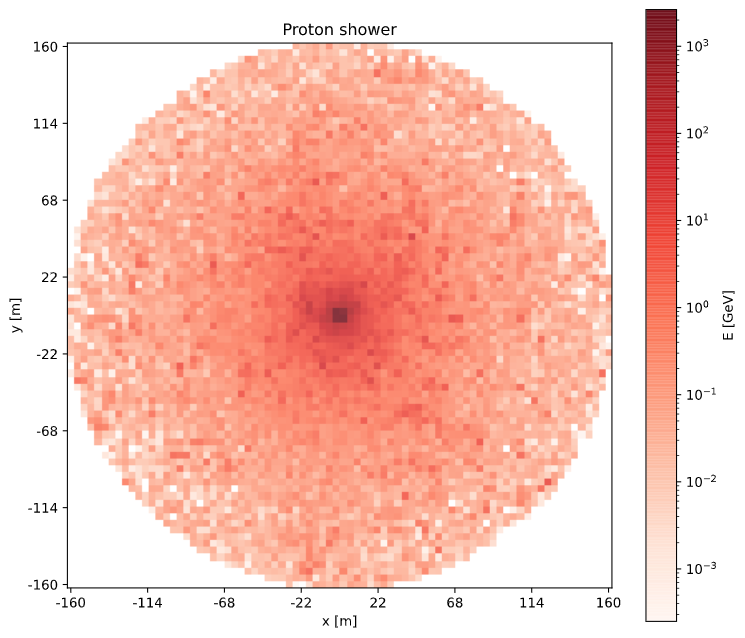
\includegraphics[width=\textwidth]{imagenes/01_Introduccion/proton.png}
         \caption{Cascada generada por protones}
         \label{fig:three sin x}
     \end{subfigure}
        \caption{Muestras del conjunto de datos}
        \label{fig:three graphs}
\end{figure}

Estas imágenes (y las demás que componen el conjunto de datos) han sido generadas usando el simulador CORSIKA, por lo tanto no es necesario el preprocesamiento de estas imágenes ya que los simuladores generan datos más limpios aunque modelen un ruido \cite{hapnote}.\\

Pero ¿para qué necesitan estos datos simulados? Sirven para hacer pruebas de concepto del próximo observatorio de rayos gamma que se va a construir en Sudamérica a una altitud de 4.4 km mínimo. Al ser un proyecto millonario (con un coste estimado de 40-50 millones de euros) se espera que tenga buenos resultados en el campo de investigación de la física de partículas y que esté en funcionamiento por 20 años. Por tanto, no sería lo más indicado construir el observatorio sin hacer pruebas ya que en caso de no sacar buenos resultados sería un derroche de dinero y de tiempo para bastantes investigadores. Este observatorio está planeado para ser construido completamente en 4 fases \cite{hapnote}:

\begin{itemize}
    \item Fase 1: cubrir un área de 20.000m$^2$ con un factor de llenado alto para dar resultados únicos en bajas energías.
    \item Fase 2: cubrir un área de 1km$^2$ con un factor de llenado bajo para dar resultados únicos en altas energías.
    \item Fase 3: cubrir un área de 80.000m$^2$ con un factor de llenado alto para dar resultados únicos en bajas energías.
    \item Fase 4: cubrir un área de 1km$^2$ con un factor de llenado bajo para dar resultados únicos en altas energías.
\end{itemize}

A continuación, en la siguiente Figura se puede observar la disposición del \textit{array} de \textit{Water Cherenkov Detectors} tal y como está planificada.\\

\begin{figure}[H]
	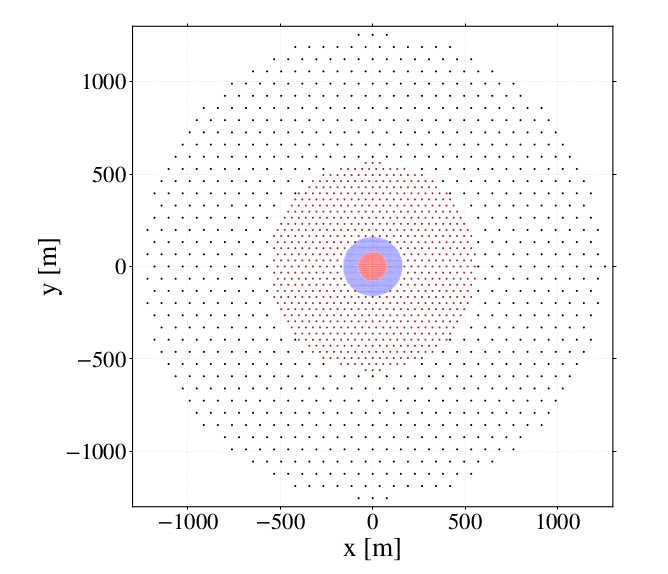
\includegraphics[width=1.\linewidth]{imagenes/01_Introduccion/layout.png}
	\centering
	\caption{Disposición planificada para los WCD. Las fases están pintadas, en orden, en los colores rojo, marrón, azul y negro respectivamente \cite{hapnote}.}
	\label{fig:wcdschema}
\end{figure}

\section{Análisis del Conjunto de Datos}\label{chap:datanalysis}

En este capítulo se muestra el \textit{Jupyter notebook} desarrollado para realizar el análisis de los datos, junto con comentarios de los resultados obtenidos.

\includepdf[pages=-]{data_analysis.pdf}
